\section*{Our implementation of the Particle Filter}
An implementation of the Particle Filter consists mainly of designing the probability functions $\cprobnext{X}$ and $\cprob{I_n}{X_n}$, and providing the algorithm with a sensible initialization. This is what this project is all about. The rest just consists of taking samples from these functions.

\subsection*{The prediction step: The Database}

We investigate the plausibility of implementging $\cprobnext{X}$ as a search through a database of training data. We set up a database of known transitions between whisker shapes. A transition $T$ consists of a ``from'' state $f$ and a''to'' state $t$. This denotes that ``we have observed with 100\% accuracy that a whisker went from this shape to that shape in one time step''. We then approximate $\cprobnext{X}$ as a weighted average of the database, where transitions are weighted by how much their ``from'' parts differ from the hypotheses in $X_n$.

What we do in practice when sampling is: for each hypothesis $x_n^i \in X_n$,

\begin{enumerate}
  \item For each transition $T^j = (f^j, t^j)$ in the database, calculate the function $d^{ij}$ that is the difference between the two functions described by $x_n^i$ and $f^j$. In this case, both are polynomials and thus $d^{ij}$ is the polynomial with coefficients given by the tuple $x_n^i - f^i$.
  \item Let $w^{ij} = \left(\frac{1}{\norm{d^{ij}}_{\Ltwo}}\right)^a$, the reciprocal of the $\Ltwo$ norm of $d^{ij}$ raised to a power $a$.
  \item Return $\frac{\sum_j t^j w^{ij}}{\sum_jw^{ij}}$, the weighted average of the ``to'' states with weights $w^{ij}$.
\end{enumerate}

Doing this for each hypothesis $x_n^i$ yields the set $\bar{X}_n$. We have not yet thoroughly investigated how the power $a$ qualitatively affects the tracking results, but $a=4$ seems to be a good value.

\subsection*{The filtering step: Image comparison}

\begin{figure}
  \centering
  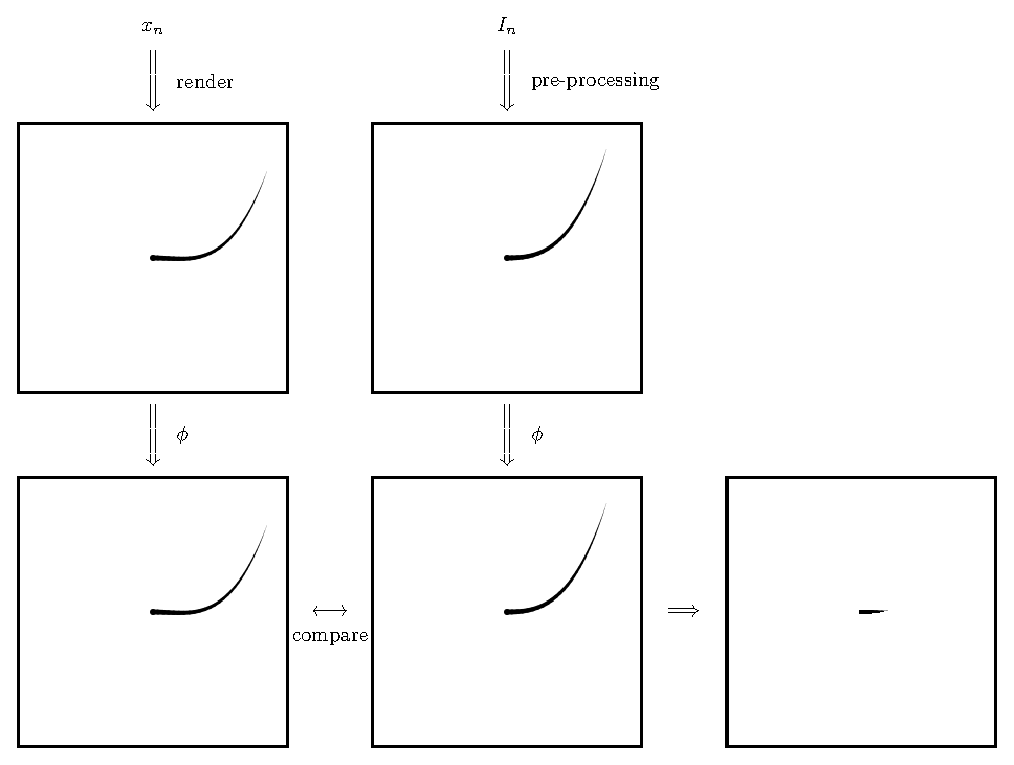
\includegraphics[scale=1.0]{whisker_compare.pdf}
  \caption{Schematic image of the process to evaluate the importance of a hypothesis.}
  \label{fig:whisker_compare}
\end{figure}

We implement the probability function $\cprob{I_n}{X_n}$ as simply checking if the image pixels beneath the whiskers $X_n$ look like whisker pixels. The image $I_n$ is grayscale, and so each pixel can be identified with a number between 0 and 255, inclusive. We assume that whisker pixels have a high value and background pixels have a low value.

We first preprocess the image using a transformation $\phi$, to make the measurement easier. At the current stage in our testing, the images used are generated synthetic ones that are already easy to process. Therefore we let $\phi$ be the identity transformation at the moment.

After preprocessing the image, for each hypothesis $\bar{x}_n^i \in \bar{X}_n$ we create a \emph{mask} image $I_n^i$. This image will be zero everywhere except where the whisker $\bar{x}_n^i$ is. We then let $w^i = \sum\limits_{\mathrm{pixels}}I_n \cdot I_n^i$, where the multiplication is done component-wise. We then let $\left\{\left(\bar{x}_n^i, w^i\right)\right\}_{i=1}^N$ define a discrete probability function that returns $\bar{x}_n^i$ with probability $w^i$, and let this distribution be our approximation of $\cprob{I_N}{X_n}$.

\begin{figure}
  \centering
  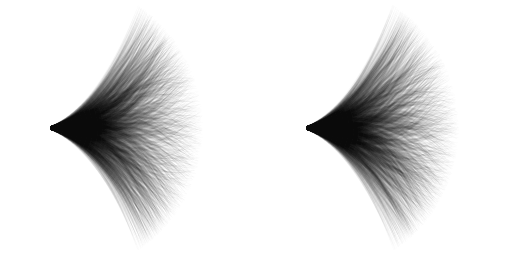
\includegraphics[width=0.7\textwidth]{database_gwhisker_spline3_n2048_from_to_fixed.png}
  \caption{View of all whiskers in transition database. Left: from-states. Right: to-states.}
  \label{fig:database}
\end{figure}

\subsection*{Example tracking image}

Figure \ref{fig:particles} shows an illustration of the three tracking steps. The blue lines are the hypotheses $\bar{X}_n$ sampled from the database. The red lines are these same hypotheses, but after resampling, $X_n$. The green line is the estimate $x_n$, the mean of $X_n$. One can see how $X_n$ is slightly more concentrated around the tracked whisker (white) than $\bar{X}_n$ is.

\begin{figure}[h]
  \centering
  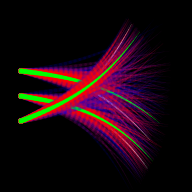
\includegraphics[width=0.3\textwidth]{tracking-particles-cropped.png}
  \caption{Tracking image with $\bar{X}_n$ (blue) and $X_n$ (blue) drawn along with the estimate $x_n$ (green).}
  \label{fig:particles}
\end{figure}

